\section{Evaluation}
\label{sec:eval}

We evaluate the deterministic core of the reference implementation: the parts of
a Trust Record whose cost and correctness do not depend on a live model or an
online attestation service. All numbers below were produced by a committed
harness (\texttt{experiments/bench.py}) run against \texttt{agentrust-trace} at
trace-spec revision 523f8cc and \texttt{trace-tests} 0.2.0 (revision 661c177);
the raw outputs are committed under \texttt{experiments/results/}. The SDK
reported version 0.2.0, but its signing code is that of release 0.3.0: release
0.2.0 canonicalizes with \texttt{json.dumps(sort\_keys=True)} and has no
\texttt{verify\_record}, so the harness cannot run against it. The five vectors
and the checker at these revisions use the v0.1 profile URI
\texttt{tag:agentrust.io,2026:trace-v0.1}; that checker rejects a record
carrying the v0.2 URI of Section~\ref{sec:model} with TR-ENV-001. Silicon
cert-chain appraisal (AMD KDS, Intel DCAP) and any LLM-in-the-loop cost are out
of scope here because they require external services or model calls, and are not
measured. Measurements were taken on a single core of an ARMv8 (Qualcomm) host
under CPython 3.12; absolute latencies are hardware-dependent and are reported to
show order of magnitude, not a hardware ranking.

\subsection{Canonicalization determinism}

A Trust Record's signature is taken over its RFC~8785 JCS canonical byte
sequence (Section~\ref{sec:model:sig}). Cross-implementation verification only
works if canonicalization is deterministic: the same logical record must yield
byte-identical output regardless of how the object was constructed. We tested
this directly by canonicalizing each of the five shipped conformance vectors 200
times, shuffling every object's key insertion order on each pass, and hashing the
result. A correct canonicalizer must produce exactly one distinct SHA-256 per
record. Across all $5 \times 200 = 1000$ canonicalizations we observed exactly 5
distinct hashes, one per record (Table~\ref{tab:eval-core}): canonicalization is
insensitive to key order and fully deterministic, as required. Shuffling key
order does not distinguish RFC~8785 from sorted \texttt{json.dumps}, and the
evaluated checker used the latter: a record with a non-ASCII \texttt{subject}
that the SDK signs and verifies fails TR-SIG at the same revisions
(\texttt{experiments/results/rerun-2026-10-01}). Later trace-tests releases
canonicalize with RFC~8785.

\subsection{Sign and verify cost}

Table~\ref{tab:eval-core} reports the end-to-end cost of the signing and
verification paths, each of which canonicalizes the record (JCS) and then runs
Ed25519. Over $5000$ iterations after a $500$-iteration warmup, signing averaged
$0.129$~ms per record (median $0.094$~ms, p99 $0.580$~ms) and verification
averaged $0.211$~ms (median $0.158$~ms, p99 $0.856$~ms), for single-core
throughputs of roughly $7{,}700$ signs/s and $4{,}700$ verifies/s.
Figure~\ref{fig:latency} shows the full per-operation latency distributions and
Figure~\ref{fig:throughput} the throughput. Sub-millisecond verification means a
relying party can appraise the deterministic core of a record inline on the
request path; the cost that matters in production is the external attestation and
transparency lookups, not the record cryptography.

\begin{table}[h]
\centering
\small
\caption{Deterministic-core measurements from \texttt{experiments/bench.py}
(agentrust-trace at 523f8cc, trace-tests 0.2.0; single core, CPython 3.12, ARMv8).
Latencies are per operation over 5000 iterations.}
\label{tab:eval-core}
\begin{tabular}{lrrrr}
\toprule
Operation & mean (ms) & median (ms) & p99 (ms) & throughput (ops/s) \\
\midrule
JCS canonicalize + sign   & 0.129 & 0.094 & 0.580 & 7{,}734 \\
JCS canonicalize + verify & 0.211 & 0.158 & 0.856 & 4{,}731 \\
\midrule
\multicolumn{5}{l}{JCS determinism: 1000 canonicalizations (5 records $\times$ 200 shuffles)} \\
\multicolumn{5}{l}{\quad distinct hashes observed: 5 (one per record) $\Rightarrow$ deterministic} \\
\bottomrule
\end{tabular}
\end{table}

\begin{figure}[h]
\centering
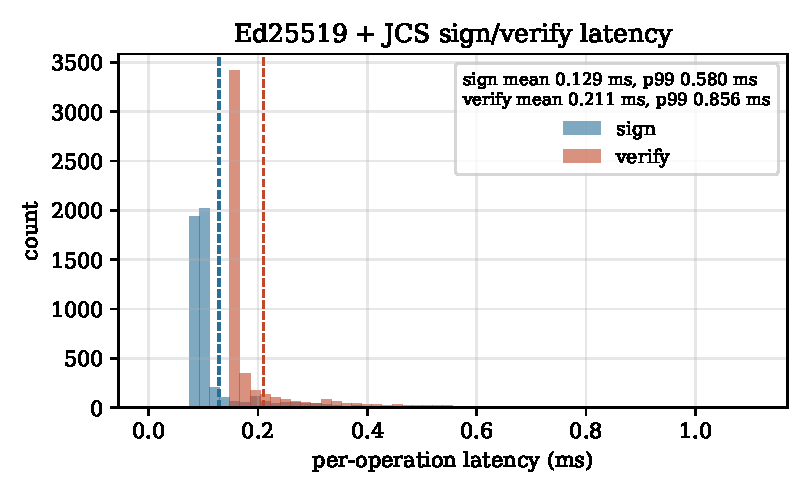
\includegraphics[width=0.72\textwidth]{figures/verify_latency.pdf}
\caption{Per-operation latency distribution for the sign and verify paths (JCS
canonicalization plus Ed25519), 5000 iterations each. Dashed lines mark the
means. Both paths are sub-millisecond in the body of the distribution, with a
short scheduler-induced tail.}
\label{fig:latency}
\end{figure}

\begin{figure}[h]
\centering
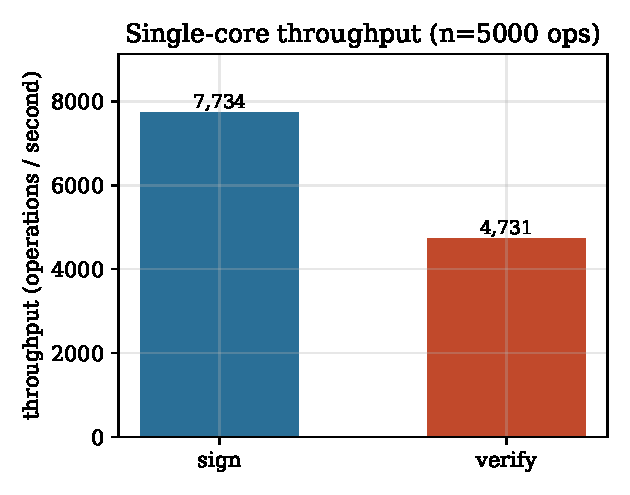
\includegraphics[width=0.52\textwidth]{figures/throughput.pdf}
\caption{Single-core throughput for the sign and verify paths. Verification is
the hot path for a relying party; at roughly $4{,}700$ verifies/s per core the
record cryptography is not the bottleneck relative to the external attestation
and transparency lookups a full appraisal also performs.}
\label{fig:throughput}
\end{figure}

\subsection{Record size}

Trust Records are compact. Table~\ref{tab:eval-size} gives the canonical
(signature pre-image) size of each shipped vector plus a synthetic, fully
populated Level~2 record. A minimal Level~0 record is under $0.9$~KB; a complete
Level~2 record with TEE measurement, SLSA provenance, tool-transcript binding,
and transparency receipt is under $1.4$~KB; the cMCP-profiled envelope, which
carries the full gateway call summary, is $1.6$~KB. The synthetic record was
measured with the v0.1 profile URI; the committed harness now emits the v0.2
URI, which is four bytes longer, and gives 1{,}389 bytes. Records this small travel with
the workload as a header or sidecar without meaningful overhead.

\begin{table}[h]
\centering
\small
\caption{Canonical (JCS, signature pre-image) size of the shipped conformance
vectors and a synthetic fully-populated Level~2 record, from
\texttt{experiments/results/record\_sizes.json}.}
\label{tab:eval-size}
\begin{tabular}{lr}
\toprule
Record & canonical size (bytes) \\
\midrule
\texttt{valid\_level0} (minimal L0)        & 878 \\
\texttt{valid\_level0\_with\_transcript}   & 1{,}109 \\
synthetic full L2 (all fields)             & 1{,}385 \\
\texttt{valid\_cmcp\_runtime} (cMCP profile) & 1{,}612 \\
\bottomrule
\end{tabular}
\end{table}

\subsection{Conformance suite behaviour}

Finally we ran the shipped \texttt{trace-tests} runner over every shipped vector
at Levels~0, 1, and 2, tallying \texttt{pass}/\texttt{fail}/\texttt{skip}/%
\texttt{unverified} findings (Table~\ref{tab:eval-conf}). The archival vectors
are unsigned test data with a 2025 \texttt{iat}, so the run disables the freshness
bound to isolate \emph{structural} conformance; TR-SIG correspondingly reports
\texttt{unverified} for the unsigned plain-trace vectors, which is the honest
expected outcome (an \texttt{unverified} record passes at Level~0 with an advisory
and fails at Level~1 and above, per Section~\ref{sec:conformance}). The two plain-trace positive vectors pass at Level~0 and fail at
Levels~1 and~2. The cMCP fixture fails at all three levels in this captured run.
The \texttt{invalid\_wrong\_profile} fixture fails at every level, while
\texttt{invalid\_missing\_runtime} passes at Level~0 and fails at Levels~1 and~2.
These are the outcomes in the committed result JSON; fixture names do not
establish the expected or observed verdict. In particular, the Level~0 pass
for the missing-runtime fixture is a limit of this historical check set,
not evidence of complete structural validation. The signed-record path is
exercised separately by the sign/verify benchmark. These results describe
the recorded package versions and do not certify the current implementation.

\begin{table}[h]
\centering
\small
\caption{Conformance findings from the shipped \texttt{trace-tests} runner
(\texttt{experiments/results/conformance.json}), reported as
pass\,/\,fail\,/\,skip\,/\,unverified. ``L0 pass'' is the suite's overall verdict
at Level~0. Freshness disabled to isolate structural conformance of the archival
vectors; unsigned plain-trace vectors report TR-SIG \texttt{unverified} by design.}
\label{tab:eval-conf}
\begin{tabular}{llccc}
\toprule
Vector & fmt & L0 (p/f/s/u) & L1 (p/f/s/u) & L2 (p/f/s/u) \\
\midrule
\texttt{valid\_level0}              & trace & 7/0/0/1 & 11/1/1/0 & 12/2/1/0 \\
\texttt{valid\_level0\_w/transcript} & trace & 7/0/0/1 & 11/1/1/0 & 14/1/1/0 \\
\texttt{valid\_cmcp\_runtime}       & cMCP  & 6/1/0/0 & 8/2/1/0  & 10/3/1/0 \\
\texttt{invalid\_missing\_runtime}  & trace & 7/0/0/1 & 9/2/0/0  & 10/3/0/0 \\
\texttt{invalid\_wrong\_profile}    & trace & 6/1/0/1 & 10/2/1/0 & 11/3/1/0 \\
\bottomrule
\end{tabular}
\end{table}
